\section{Исследовательский раздел}
\subsection{Загрузка драйвера}
Для корректного функционирования разработанного ПО необходимо
выполнить установку реализованного драйвера. Для этого сперва нужно выгрузить драйвер геймпада, что загружен по умолчанию ---
\textit{sudo rmmod xpad}. Далее уже загрузить данное ПО --- \textit{sudo insmod myxpad.ko}. На Рисунке \ref{sudo} показан данный процесс.

\begin{figure}[h!]
	\centering
	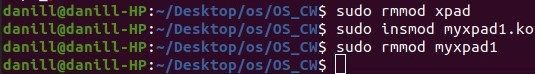
\includegraphics[scale=0.9]{img/sudo.jpg}
	\caption{Установка драйвера}
	\label{sudo}
\end{figure}\par

\subsection{Результат выполнения}
На Рисунке \ref{dmesg} показан вывод программы.
\begin{figure}[h!]
	\centering
	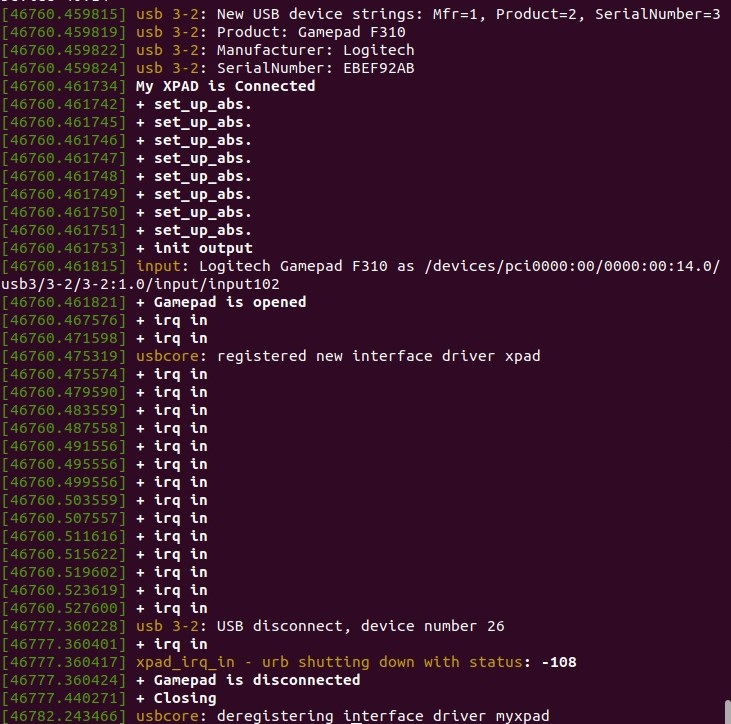
\includegraphics[scale=0.9]{img/ex1.jpg}
	\caption{Вывод программы}
	\label{dmesg}
\end{figure}\par

\pagebreak